\section{Methods}
    We have multiple goals in this experiment series:
    \begin{enumerate}
        \item The calibration of the voltmeter and its corresponding pressures.
        \item Determination of the absolute zero point of temperature.
        \item Determination of the temperature of liquid nitrogen.
    \end{enumerate}
    We will achieve these results by making use of the linearly corresponding properties of ideal gases with the help of the apparatus shown in Fig.~\ref{fig_setup}.

    \begin{figure}[H]
        \centering
        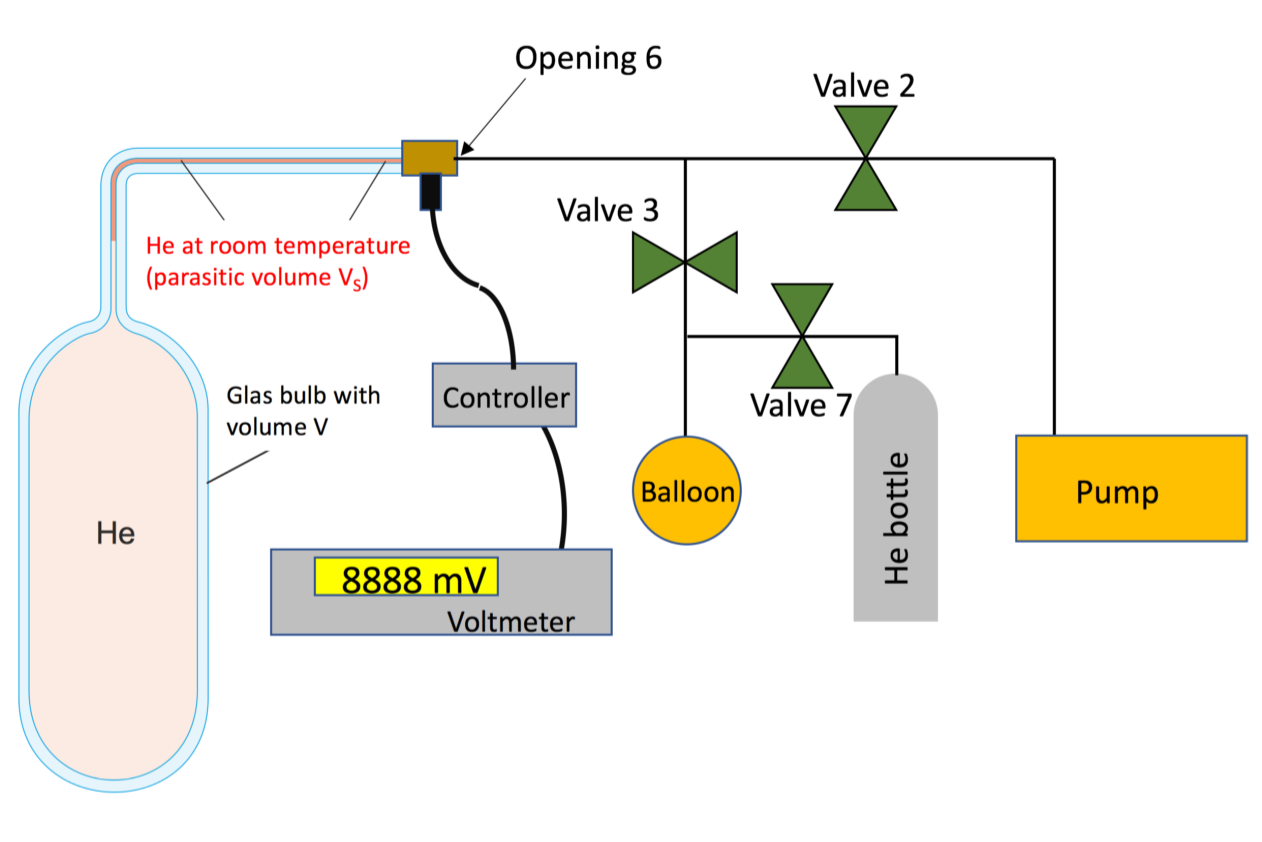
\includegraphics[]{src/images/experimental_setup.png}
        \caption{experimental setup: A glass bulb filled with helium is connected to a sensor and a system of tubes, in turn connecting to a pump, a helium bottle and a baloon.
        The sensor outputs a voltage linearly related to the applied pressure, the pump can reduce the pressure in the bulb, the helium bottle is the helium supply and the balloon acts as a pressure regulator between the bulb and the bottle.
        Multiple valves control the gas flow within the tubes.}
        \label{fig_setup}
    \end{figure}

    Starting with the calibration of the voltmeter, the voltages at room pressure and when a vacuum pump is connected are noted and compared to the actual pressure in the room and the pressure, the pump is able to maintain.
    Hereafter, the glass bulb is evacuated and filled with helium, the reason being that the properties of helium are closer to ideal gases than air.
    Moreover, the oxygen from the air would liquefy when cooled down to the temperature of liquid nitrogen (which would happen in the third step of the experiment series) and liquids do not act according to the ideal gas equation.

    In the next step, the helium-filled glass bulb is heated to the boiling point of water using steam while leaving the apparatus open so that excess helium can escape.
    We chose the temperature of boiling water as the value can easily be calculated using ambient temperature and pressure as well as tabulated data.
    The gas will only expand in this step and hence no air will get into the glass bulb.
    As soon as the helium has reached the desired temperature, the voltage is taken and the system is closed back up at opening 6. (see Fig.~\ref{fig_setup})
    From now on, the closed system can be used just like a thermometer when calculating the temperature at its corresponding voltage.
    
    To create a linear relation of pressure and temperature in the bulb, a second measurement is needed.
    The temperature at the freezing point of water is also known, so this is the second point used in our case.
    The Helium filled bulb is cooled in an ice bath and the voltage is taken.
    To calculate the absolute zero point of temperature, we have to pay respect to the expansion of the glass bulb with increasing temperature.
    Please refer to section~\ref{sec_results} for the calculation.

    As mentioned before, the closed system acts like a thermometer.
    Therefore, we can cool down the helium filled bulb using liquid nitrogen, read off the voltage and calculate the corresponding temperature of liquid nitrogen.
    In this step, the expansion of the glass bulb must be taken into account as well.

    The error sources in this experiment can be classified:
    \begin{itemize}
        \item In our analysis, it is assumed that the temperature in the room stays the same during the whole process.
        Needless to say that this does not have to be the case: small fluctuations happen naturally.
        As a result, corrupted data could occur during the calibration of the sensor.
        Furthermore, the temperature was read off an analog thermometer leading to an uncertainty caused by the limits of the human eye.
        \item Next to the temperature, the pressure does also fluctuate over time.
        The boiling point of water depends on the pressure.
        Hence, when heating the helium to the boiling point of water, a deviation in the temperature used in calculations below and the real temperature could exist.
        As with temperature, the pressure was also read off an analog measurement device and this value could slightly differ from the real pressure.
        \item The manufacturer of the sensor has defined a certain nonlinearity in the conversion of pressure to its corresponding voltage.
        \item The pump does not create an absolute vacuum and small amounts of air could stay in the glass bulb.
        This would have the biggest impact on the temperature measurement of liquid nitrogen as parts of the air would liquify and the linearity resulting from the ideal gas law eq.~\ref{eq_igl} would not be maintained.
        \item When heating and cooling the gas in the bulb, the glass itself could need more time to evenly distribute the temperature resulting in an uneven change in the gas volume, therefore changing the pressure.
        This would affect the difference between the linear approach and the exact calculation of $t_0$ and $t_{LN2}$.
    \end{itemize}
